% Please don't change anything in the documentclass below:
% We recommend using these packages as below, but if you have a good reason and want to change these, you can.
\documentclass[11pt]{article}
\usepackage{deauthor}
\usepackage{tikz}
\usetikzlibrary{shapes,arrows.meta, positioning}
\usepackage{cite}
\usepackage{amsmath,amssymb,amsfonts}
\usepackage{graphicx}
\usepackage{textcomp}
\usepackage{xcolor}
\usepackage{booktabs}
\usepackage{subcaption}
\usepackage{soul}
\usepackage{float}
\usepackage{algpseudocode}
\usepackage{algorithm2e}  % Remove if you don't need algorithm2e
\usepackage{enumitem}
\usepackage{tikz}
\usepackage{blindtext}
\usepackage{hyperref}
\hypersetup{
    colorlinks=true,
    linkcolor=blue,
    filecolor=magenta,      
    urlcolor=cyan,
    pdftitle={Overleaf Example},
    pdfpagemode=FullScreen,
    }
\usepackage{url}


\urlstyle{same}


\begin{document}

\title{\textsf{G-VARS}: Towards Personalized Risk Assessments by Analyzing Gun Violence Susceptibility with Personal Knowledge Graphs}

% Submissions should be anonymized. See the CFP for details on how to anonymize your paper, including any references to your own work.
%\author{\em Anonymous Authors}

% The author information is skipped here, but can be used to include author information in the publication.
\author{Dipkamal Bhusal$^{1}$~~~~~~Sara Rampazzi$^{2}$~~~~~~Michael Clifford$^{3}$~~~~~~Nidhi Rastogi$^{1}$\\ \\
%Affiliation
$^1$Rochester Institute of Technology, NY, USA\\
$^2$University of Florida, FL, USA\\
$^3$Toyota InfoTech, CA, USA
}

\maketitle

\thispagestyle{plain}
\pagestyle{plain}

\begin{abstract}
Gun violence is a concerning issue in the United States and requires immediate societal attention for improved prediction and prevention. Prior approaches have often overlooked mental health, relying on static factors such as age, gender, and the criminal history of the crime perpetrator. These approaches frequently fail to consider the context and environmental factors contributing to an individual’s risk of gun violence. In this paper, we propose \textsf{G-VARS}, a framework based on personal knowledge graphs that aggregates public and personal information to assess and evaluate individuals for potential gun violence. \textsf{G-VARS} comprises three phases: data collection, personal knowledge graph generation, and personalized risk assessment and intervention planning. We also present a case study where we apply the \textsf{G-VARS} framework to assess the risk of gun violence among urban youth.

\end{abstract}

\section{Introduction}
Gun violence is a critical public health issue in the United States. In 2023, the US broke the record for the maximum number of mass shootings in a year \cite{michael_2023}. According to the Centers for Disease Control and Prevention (CDC), approximately 48,000 gun-related deaths occurred in 2022, which averages to 132 people dying from a firearm-related injury each day~\cite{CDC}. Predicting and preventing gun violence is a multifaceted challenge, and traditional risk assessment models have several limitations. For instance, prior approaches rely on static factors like age, gender, and criminal history of the crime perpetrator \cite{smith2020limitations} and frequently fail to consider the context and environmental factors contributing to an individual's risk of gun violence \cite{jones2019contextual}. Mental health factors are often overlooked, which misses the crucial role they play in risk assessment \cite{doe2021mental}. Additionally, prior approaches do not adapt to changing circumstances. To address these issues, there is a growing interest in more advanced, personalized, and dynamic approaches to gun violence risk assessment, such as machine learning and predictive analytics \cite{chen2020machine}, social media monitoring \cite{adams2019social}, mental health screening \cite{lee2020screening}, and community-based strategies \cite{harris2022community}.
\par
In this paper, we propose the Gun Violence Assessment and Risk Stratification (G-VARS) framework based on Personal Knowledge Graphs (PKG). A PKG is a structured, user-centric graph connected to nodes (also called entities) via edges (also called relations), which provide knowledge about an individual that is of personal importance~\cite{balog2019personal}. In the context of assessing risks from Gun Violence, a PKG is a structured representation of an individual's unique circumstances and risk factors, capturing the interplay between individual, social, and environmental factors, enabling the analysis of gun violence risk factors and the development of personalized risk assessments. \textsf{G-VARS} can be utilized by various stakeholders, including healthcare providers can use it to evaluate potential violence risks, while law enforcement agencies can use it for risk identification and intervention planning. It can also help in fighting the inflow of illicit weapons used in crimes. Policymakers can leverage \textsf{G-VARS} for data-driven insights into the root causes of gun violence, informing policy decisions. Research institutions can utilize it to understand gun violence factors and develop prevention strategies. Lastly, community organizations can use \textsf{G-VARS} to create tailored interventions based on specific risk factors. The actual implementation of \textsf{G-VARS} is no trivial task, and we answer some of these challenges in this paper through detailed planning and considerations, especially related to ethical and privacy aspects. We envision that the \textsf{G-VARS} will have the following use cases:
\newline
\textit{(1) Identifying individuals at high risk of gun violence}: The PKG can be used to identify individuals who are at high risk of perpetrating or being a victim of gun violence. This information can then be used to intervene with these individuals and provide them with the support they need.
\newline
\textit{(2) Developing targeted interventions}: The PKG can be used to develop targeted interventions for individuals at high risk of gun violence. These interventions can include mental health treatment, substance abuse treatment, and violence prevention programs.
\newline
\textit{(3) Informing policy decisions}: The PKG can be used to inform policy decisions about gun violence prevention. For example, the PKG can be used to identify areas where there is a high risk of gun violence and to develop targeted interventions for those areas.

\subsection*{Privacy and Ethics Concerns}
Building and analyzing \textsf{G-VARS} is a complex task. Aggregating personal, familial, and social data with health information raises significant privacy and ethical concerns. Consequently, finding and collecting sufficient data for predictions while upholding ethical and legal frameworks presents a significant challenge \cite{lee2016ethical,nissenbaum2020protecting,ieee_privacy,USCommerce}. However, advancements in privacy research and increased collaboration between governments, healthcare institutions, and other stakeholders offer a promising path forward. 
For instance, the Open Knowledge Network (OKN) initiative by the NSF \cite{nsf_proto_okn_nsf23571,okn_2022}, an interconnected network of knowledge graphs, could provide a crucial public data infrastructure to facilitate an AI-driven future. This network would enable the integration of diverse data necessary for the development of solutions to drive sustained economic growth, broaden opportunities, and tackle complex problems ranging from climate change to social equity. Addressing gun violence is a principal theme of this initiative. In conjunction with this, the National Institute of Justice (NIJ)\cite{nij_gun_violence} is endeavoring to develop a comprehensive database for nonfatal firearm injuries to inform evidence-based prevention policies and demonstrate efforts toward building a data infrastructure for AI-driven solutions. This paper operates under the assumption that such a knowledge network will be operational in the near future, paving the way for exciting research directions that will benefit society.

\section{Background and Related Work}\label{sec:background}
\subsection{Personal Knowledge Graphs (PKG)}
A Personal Knowledge Graph (PKG) is a resource of structured information about entities personally related to an individual, its attributes, and the relations between them \cite{balog2019personal} (see Figure \ref{fig:pkg}). Using this format, a PKG organizes an individual's personal data, including education, work history, hobbies, relationships, and preferences, into a structured format \cite{rastogi2020personal}. It connects these elements, highlighting relationships and patterns, to create a comprehensive overview of an individual's knowledge and experiences. In the context of this paper, a PKG is a structured representation of an individual's unique circumstances and risk factors, capturing the interplay between individual, social, and environmental factors, enabling the analysis of gun violence risk factors and the development of personalized risk assessments. We can leverage a PKG for personalized risk assessments by integrating and analyzing relevant data points such as an individual's mental health history, social connections, geographic location, and exposure to violence \cite{rastogi2020personal} within the context of gun violence risk factors. This analysis can further provide insights into an individual's susceptibility to gun violence. Using machine learning algorithms, we can then process this data to generate risk assessments that are more accurate and context-aware, enabling targeted interventions and prevention strategies tailored to the individual's unique circumstances.

\begin{figure}[h]
\small
\centering
\resizebox{1\columnwidth}{!}{
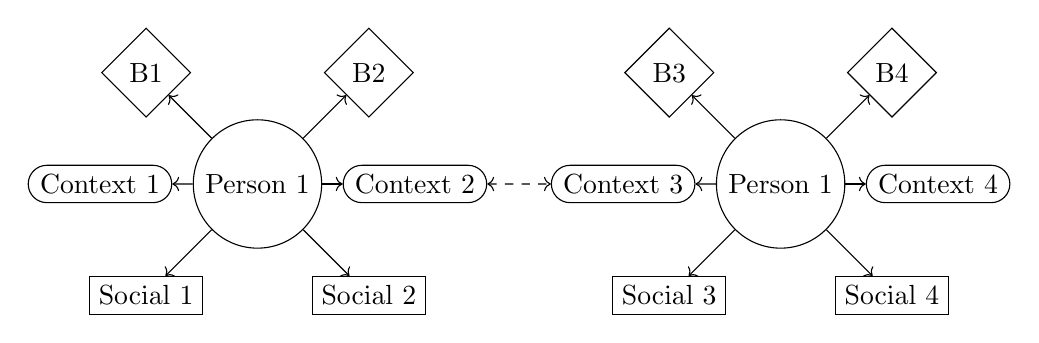
\begin{tikzpicture}[node distance=2cm, auto]

  % PKG 1
  \node[circle, draw, minimum size=0.75cm] (PKG1) {Person 1};
  \node[rectangle, draw, below left of=PKG1] (Social1) {Social 1};
  \node[rectangle, draw, below right of=PKG1] (Social2) {Social 2};
  \node[diamond, draw, minimum size=0.35cm, above left of=PKG1] (Behavior1) {B1};
  \node[diamond, draw, minimum size=0.35cm, above right of=PKG1] (Behavior2) {B2};
  \node[rounded rectangle, draw, left of=PKG1] (Context1) {Context 1};
  \node[rounded rectangle, draw, right of=PKG1] (Context2) {Context 2};

  \draw[->] (PKG1) -- (Social1);
  \draw[->] (PKG1) -- (Social2);
  \draw[->] (PKG1) -- (Behavior1);
  \draw[->] (PKG1) -- (Behavior2);
  \draw[->] (PKG1) -- (Context1);
  \draw[->] (PKG1) -- (Context2);

  % PKG 2
  \node[circle, draw, minimum size=0.75cm, right=5cm of PKG1] (PKG2) {Person 1};
  \node[rectangle, draw, below left of=PKG2] (Social3) {Social 3};
  \node[rectangle, draw, below right of=PKG2] (Social4) {Social 4};
  \node[diamond, draw, minimum size=0.35cm, above left of=PKG2] (Behavior3) {B3};
  \node[diamond, draw, minimum size=0.35cm, above right of=PKG2] (Behavior4) {B4};
  \node[rounded rectangle, draw, left of=PKG2] (Context3) {Context 3};
  \node[rounded rectangle, draw, right of=PKG2] (Context4) {Context 4};

  \draw[->] (PKG2) -- (Social3);
  \draw[->] (PKG2) -- (Social4);
  \draw[->] (PKG2) -- (Behavior3);
  \draw[->] (PKG2) -- (Behavior4);
  \draw[->] (PKG2) -- (Context3);
  \draw[->] (PKG2) -- (Context4);

  % Connecting edge between Context 2 of PKG 1 and Context 3 of PKG 2
  \draw[<->,dashed] (Context2) -- (Context3);

\end{tikzpicture}
}
\caption{Personal Knowledge Graphs of Person 1 \& Person 2 and their different components. \textit{Social} nodes symbolize social networks relevant to each PKG. \textit{Behavioral} nodes (B1, B2) indicate behavior patterns for each person. \textit{Context} nodes are the environmental, situational factors influencing each person. Person 1 \& 2 are connected due to overlapping context.}
\label{fig:pkg}
\end{figure}


\subsection{Limitations of Traditional Risk Assessment Models for Gun Violence}
\textbf{Data-Driven Limitations:} One set of limitations involves the data-driven aspects of these models. Traditional approaches often rely on static variables such as age, gender, and criminal history for risk assessment, which may lead to low predictive accuracy \cite{smith2020limitations}. Furthermore, these models tend to overlook contextual factors, including socioeconomic status, access to firearms, and exposure to community violence, which are crucial in assessing an individual's risk \cite{jones2019contextual}. Additionally, mental health considerations, although significant contributors to violence, are inadequately incorporated into these models \cite{doe2021mental}. Moreover, bias and discrimination are concerns, as these models may disproportionately affect certain demographic groups, leading to over-policing and inequities in the criminal justice system \cite{Lum_2016}. Finally, the inability of traditional models to predict rare events, such as gun violence by individuals with no prior violent history, poses significant challenges gun violence among certain demographic groups, such as people of color or those with mental health diagnoses \cite{Lum_2016}.\\
\textbf{Lack of consideration for protective factors:} Traditional risk assessment models often focus on identifying and assessing risk factors, but they may not adequately consider the role of protective factors. Protective factors are characteristics or circumstances that can reduce the likelihood of gun violence, such as strong social support, access to mental health care, or participation in positive activities \cite{Kovacs_2019}.\\
\textbf{Limited predictive accuracy:} Traditional risk assessment models have shown limited predictive accuracy, meaning that they are not always able to accurately identify individuals who are at risk of committing gun violence. This lack of accuracy can lead to both false positives (individuals who are incorrectly identified as being at risk) and false negatives (individuals who are at risk but are not identified by the model) \cite{Fazel_2020}.\\
\textbf{Operational Challenges:} Operational limitations also plague traditional risk assessment models. These models typically offer static assessments that do not adapt to changing circumstances or behaviors \cite{smith2020limitations,jones2019contextual}. Data sharing among various agencies and organizations is often limited, hindering the development of comprehensive risk assessment models \cite{Johnson_2019}. Privacy concerns arise when sensitive data is collected and shared for risk assessment, necessitating a balance between public safety and privacy rights \cite{Johnson_2019}. Resource constraints further limit scalability, as these models require substantial resources for effective implementation \cite{Davis_2020}. Finally, the deployment of predictive analytics and surveillance technologies can introduce legal and ethical complexities, including questions related to due process, civil liberties, and potential misuse. Addressing these limitations necessitates a transition towards more advanced, personalized, and context-aware approaches to gun violence risk assessment.


\subsection{Personal Knowledge Graphs for Personalized Risk Assessment}
Personal knowledge graphs (PKGs) offer a promising avenue for personalized risk assessment~\cite{Brown2018}. PKGs are representations of an individual's social, behavioral, and contextual information, capturing their unique relationships and experiences~\cite{jones2019contextual}. By analyzing PKGs, researchers can extract dynamic risk factors that may not be readily captured by traditional methods~\cite{jones2019contextual}. A growing body of research has explored the use of PKGs for risk assessment in various domains, including criminal justice~\cite{Brown2018}, child welfare~\cite{jones2019contextual}, and healthcare. These studies have demonstrated the potential of PKGs to identify individuals at high risk of recidivism~\cite{Brown2018}, child maltreatment~\cite{jones2019contextual}, and disease exacerbations. Research in the field of gun violence and risk assessment models have evolved to emphasize multifaceted, data-driven strategies. Studies supported by the National Institute of Justice (NIJ) highlight the effectiveness of such approaches in reducing gun trafficking and shootings \cite{nij2021}. Particularly noteworthy is the research on youth firearm involvement in New York City, revealing that fear and the desire for physical safety, more than criminal intent, drive young people to carry and use firearms \cite{nij2021youth}. Furthermore, studies have examined the transition from youth firearm involvement to adult criminal behaviors, offering insights into the long-term impacts of early exposure to gun violence \cite{nij2021delinquent}.

\subsection{Previous Studies on Graph Link Prediction}
Graphs are often used to model the complex network structures of real-world systems \cite{kazemi2018simple,ding2022data}. In these graphs, each node can develop various types of relationships (edges) with other nodes \cite{nasiri2022impact}. Predicting these nodes and their relationships is a key area of research, offering significant insights for diverse applications \cite{cen2019representation,kumar2022link,wang2021self,10004751}. Current methods focus on learning the significance of a node and its one- and multi-hop neighbors in a heterogeneous network graph. These approaches include using a global feature generator for initial node representations \cite{cen2019representation, kumar2022link} and a localized, attention-driven method for fine-tuning specific subgraphs \cite{wang2021self}. Additionally, some methods utilize node centralities to understand a network’s local, quasi-local, and global structures \cite{kumar2022link}. Heterogeneous social networks, characterized by their diverse interaction types and missing links (edges), present challenges for the predictive performance of existing models. To address this, \cite{10004751} propose the MTTM (Multi-Type Transferable Method) for missing link prediction. This method leverages adversarial neural networks to maintain robustness against varying types of data. Furthermore, some strategies incorporate the causal relationship between the graph structure and links to capture essential factors for accurate missing link prediction \cite{zhao2022learning}.

\subsection{Limitations in Current Research}
Despite the promising potential of PKGs, limited studies have investigated the use of PKGs for gun violence risk assessment or have focused on relatively small sample sizes~\cite{Fazel} due to which the effectiveness of PKGs in predicting gun violence risk across diverse populations remains unclear~\cite{Fazel}. Theoretical generalizations about the circumstances leading to firearms violence are notably lacking \cite{nij2021gaps}. A gap we aim to fill is the application of PKGs in the context of gun violence risk assessment by providing a more nuanced understanding of individual susceptibilities to gun violence. Our study aims to address these gaps by conducting a comprehensive analysis of gun violence risk factors using PKGs. By leveraging a large and diverse dataset, our study aims to identify novel risk factors and develop a more accurate and personalized risk assessment model. The findings of our study have the potential to inform the development of effective gun violence prevention interventions.

%\section{Motivation}\label{sec:motivation}

%\section{Datasets for Studying Gun Violence}
\section{Proposed Framework}
In this paper, we propose ``\textsf{G-VARS}'' (\ul{G}un \ul{V}iolence \ul{A}ssessment and \ul{R}isk \ul{S}tratification) Framework that uses personal knowledge graphs to analyze gun violence and the associated risks. The framework is a systematic approach to leverage individual-specific data for more accurate risk assessments related to gun violence. The framework \textsf{G-VARS} encompasses three key phases: data collection and integration, PKG construction, and personalized risk assessment and intervention planning. \textsf{G-VARS} offers several advantages over traditional risk assessment approaches, such as capturing the unique circumstances and risk profiles of individuals, enabling more accurate and targeted risk assessments; providing a holistic view of an individual's risk factors, considering individual, social, and environmental factors; enabling continuous monitoring and risk assessment by dynamically updating the knowledge graph as new data becomes available, and informing the development of tailored interventions that address the specific risk factors of each individual. Next, we describe the three key phases of \textsf{G-VARS}:

\subsection*{Phase 1: Data Collection and Integration}
In the initial phase of the \textsf{G-VARS} framework, data collection and integration are paramount but will necessitate careful consideration of ethical, privacy, and legal concerns. While diverse data from medical records, social media activity (anonymized), historical records, and environment (collected as group statistics) will be gathered to construct individual profiles, informed consent, algorithmic bias, transparency, data security, and legal compliance will be performed wherever necessary. Recognizing these challenges and that not all data points will be available at all times, a subset of the data will be used to construct the PKGs. We extensively cover the ethical, privacy and legal challenges in Section \ref{ethics} The amalgamation of this multifaceted data forms the foundation for constructing Personal Knowledge Graphs (PKGs) to enhance gun violence risk assessments.

\begin{enumerate}
\item \textbf{Demographics}: Age, gender, location, and socioeconomic status can all play a role in the risk of gun violence \cite{OToole_2023,kegler2023notes}. For instance, studies have shown that gun violence disproportionately affects racial and ethnic minorities and is highly concentrated in a relatively small number of neighborhoods that have historically been under-resourced and racially segregated \cite{CDC_2023}. Men account for 86\% of all victims of firearm death and 87\% of firearm injuries \cite{edmund2022gun}. However collecting demographics should balance the need for data with the protection of individual rights and the responsible use of technology. By focusing on group statistics, utilizing anonymized data, and contextualizing individual data, we can gain valuable insights into violence patterns while ensuring a just and ethical approach to risk assessment.

\item \textbf{Behavioral Factors}: This includes past criminal behavior, substance abuse issues, or involvement in violent incidents \cite{efsgv_2020,wamser2021understanding}. Research suggests that individuals who have been victimized by a weapon as adolescents are between two and three times more likely to perpetuate firearm violence as adults \cite{Adolescent_gun_violence}. Also, those with access to a firearm during adolescence are far more likely to perpetuate firearm violence as an adult \cite{Adolescent_gun_violence}.

\item \textbf{Mental Health}: Information about a person's mental health history, including any diagnoses or treatments, can be relevant \cite{Ramchand2021-iz,Russell2022-kq,noauthor_2021-yq}. While mental illness contributes to only about 4\% of all violence, the contribution to gun violence is even lower \cite{noauthor_2021-yq}. However, suicide risk is indeed elevated among people with certain mental illnesses (e.g., schizophrenia, depression, borderline personality disorder, bipolar disorder, and anxiety disorders), but suicide among those with such diagnoses is still rare \cite{Ramchand2021-iz}. Important to note that concerns about potential bias, discrimination, and stigma necessitate careful handling of this information. 

\item \textbf{Access to Firearms}: Details about a person's access to firearms, such as ownership or proximity to others who own guns, can be crucial \cite{noauthor_2021-fg,Adolescent_gun_violence,noauthor_2022-qy}. Studies show that access to firearms doubles the risk of homicide \cite{noauthor_2022-qy}. Simply having a gun in one's home doubles the chance of dying by homicide and increases the likelihood of suicide death by over three-fold \cite{noauthor_2021-fg}.

\item \textbf{Social Networks}: The relationships and associations a person maintains can influence their risk level \cite{tracy2016transmission,Mcdonald2013-ji,papachristos2014network}. This can include family, friends, or affiliations with certain groups. A person's social network is a key predictor of whether an individual will become a victim of gun homicide, even more so than race, age, gender, poverty, or gang affiliation \cite{Mcdonald2013-ji,papachristos2014network}.

\item \textbf{Online Activity}: Public posts or interactions on social media platforms can provide insights into a person's state of mind or intentions \cite{Written_Bynbsp_Dr2023-zu}. Studies have suggested that social media has contributed to the rise and proliferation of gun violence across the country by encouraging imitative behaviors, provoking retaliative actions, and offering ``bragging rights'' in some online communities \cite{Written_Bynbsp_Dr2023-zu}. In addition, social media has made private information such as real-time locations, personal violent imagery and discourse, and gang threats and affiliations easily accessible to the public.
\end{enumerate}

\begin{figure}[h]
\small
\centering
\resizebox{1\columnwidth}{!}{
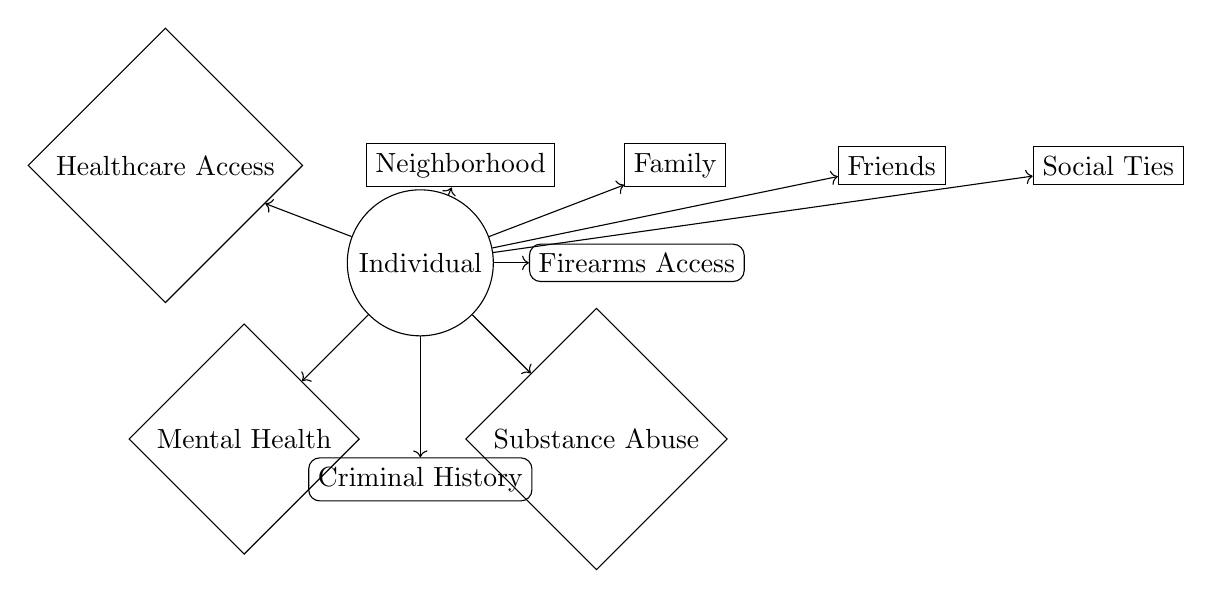
\begin{tikzpicture}[node distance=1.75cm, auto]

 % Central node 'Individual' as a circle
  \node[circle, draw] (Individual) {Individual};

  % Smaller diamond-shaped nodes for 'Mental Health', 'Substance Abuse', and 'Healthcare'
  \node[diamond, aspect=1, draw, minimum size=.5cm, below left of=Individual, xshift=-1cm, yshift=-1cm] (MentalHealth) {Mental Health};
  \node[diamond, aspect=1, draw, minimum size=.5cm, below right of=Individual, xshift=1cm, yshift=-1cm] (SubstanceAbuse) {Substance Abuse};
  \node[diamond, aspect=1, draw, minimum size=.5cm, above left of=Individual, xshift=-2cm] (Healthcare) {Healthcare Access};

  % Curved rectangle-shaped nodes for 'Firearms' and 'Criminal History'
  \node[rectangle, rounded corners, draw, below of=Individual, yshift=-1cm] (CriminalHistory) {Criminal History};
  \node[rectangle, rounded corners, draw, right of=Individual, xshift=1cm] (FirearmsAccess) {Firearms Access};

  % Rectangle-shaped nodes for 'Family', 'Friends', 'Social Ties', and 'Neighborhood'
  \node[rectangle, draw, above right of=Individual, xshift=2cm] (Family) {Family};
  \node[rectangle, draw, right of=Family, xshift=1cm] (Friends) {Friends};
  \node[rectangle, draw, right of=Friends, xshift=1cm] (SocialTies) {Social Ties};
  \node[rectangle, draw, right of=Healthcare, xshift=2cm] (Neighborhood) {Neighborhood};

  % Edges representing relationships
  \draw[->] (Individual) -- (MentalHealth);
  \draw[->] (Individual) -- (SubstanceAbuse);
  \draw[->] (Individual) -- (CriminalHistory);
  \draw[->] (Individual) -- (Family);
  \draw[->] (Individual) -- (Friends);
  \draw[->] (Individual) -- (SocialTies);
  \draw[->] (Individual) -- (Neighborhood);
  \draw[->] (Individual) -- (Healthcare);
  \draw[->] (Individual) -- (FirearmsAccess);

\end{tikzpicture}}
\caption{PKG Construction in the context of gun violence risk assessment. It incorporates Individual Factors, Social Factors, and Community Factors.}
\label{fig:pkg-construction}
\end{figure}

\subsection*{Phase 2: PKG Construction}
The construction of Personal Knowledge Graphs (PKGs) includes entities such as individuals, family members, friends, community factors, and risk factors are represented as nodes within the PKG (see Figure \ref{fig:pkg-construction}). Relationships are the connections, interactions, and influence among these entities. For instance, the individual is linked to family members, friends, community factors, and risk factors, allowing for a comprehensive representation of their social and environmental context. To attribute significance to relationships, weights are assigned based on their relative importance in predicting gun violence risk; for example, strong connections to known gang members carry higher weights than distant ties to casual acquaintances. This phase transforms raw data into a structured, interconnected graph that forms the basis for subsequent personalized risk assessments.

\textbf{Identify Entities: }The nodes in the personalized knowledge graph (PKG) represent the various entities that contribute to an individual's risk of gun violence. Therefore, the first step is to identify the entities that will be part of PKG. In the context of gun violence risk assessment, these entities can be further categorized into three main groups: (1) \textit{Individual Factors}: These nodes represent the individual's personal characteristics and background, including demographic factors (age, gender, race, ethnicity), mental health factors (diagnoses, treatment history, symptoms), substance abuse factors (types of substances used, frequency of use, treatment history), and criminal history factors (types of offenses, dates of offenses, legal consequences); (2) \textit{Social Factors}: These nodes represent the individual's social connections and environment, including family members, friends, and other social ties. The characteristics and risk factors associated with these relationships are also captured, such as exposure to violence, gang involvement, and social support networks; and (3) \textit{Community Factors}: These nodes represent the individual's community context and surroundings, including neighborhood crime rates, poverty levels, access to mental health care, and access to firearms. These factors can significantly influence an individual's risk of gun violence exposure or involvement.

\textbf{Define Relationships: }The edges in the PKG represent the connections and relationships between the various nodes. Therefore, next, we define the relationships between these entities, which can be categorized into four main types: (1) \textit{Direct Relationships}: These edges directly connect individuals to their family members, friends, and other social connections. They represent the immediate and tangible connections within an individual's social network; (2) \textit{Indirect Relationships}: These edges connect individuals to community factors, such as living in a high-crime neighborhood or having easy access to firearms. They represent the broader environmental and contextual factors that influence an individual's risk profile; 
(3) \textit{Influential Relationships}: These edges represent the strength and influence of relationships between nodes. Stronger relationships, such as close family bonds or involvement in influential social groups, carry more weight in the risk assessment process; and (4) 
\textit{Risk Factor Relationships}: These edges connect risk factors directly to individuals. Weights are assigned to these edges based on the relative importance of each risk factor in predicting gun violence risk. This allows the PKG to identify the most significant contributing factors to an individual's overall risk profile.

The collected data is finally structured in a graph format following the entities and relationships defined in the previous steps. Each entity becomes a node in the PKG, and each relationship becomes an edge connecting two nodes. Once the PKG is built, we can analyze it to identify patterns, assess risks, or generate insights (see Phase \ref{phase3}). The center of this personal knowledge graph, it would be the individual who is being assessed for the risk of gun violence\cite{ilkou2022personal}. All other entities (demographics, behavioral factors, mental health history, etc.) are connected to this central node, forming a ``spiderweb'' layout5. This allows for a personalized representation of data and interests- \cite{balog2019personal,ilkou2022personal,chakraborty2022personal}.



% (8) Integrating Siloed Personal Knowledge Graphs - Medium. https://dmccreary.medium.com/integrating-siloed-personal-knowledge-graphs-d0e68bd06685.
% (9) AI Knowledge Graph Generator | Taskade. https://www.taskade.com/generate/content/knowledge-graph.
% (10) undefined. https://doi.org/10.1145/nnnnnnn.nnnnnnn.
% (11) undefined. https://doi.org/10.1145/3341981.3344241.

\subsection*{Phase 3: Personalized Risk Assessment and Intervention Planning}\label{phase3}
This phase of the \textsf{G-VARS} framework focuses on personalized risk assessment and intervention planning. Machine learning algorithms can be used to analyze the PKG to generate a personalized risk score for each individual, indicating their likelihood of perpetrating or being a victim of gun violence. Key risk factors contributing to an individual's risk profile are identified through an analysis of node centrality and relationship weights within the PKG. This comprehensive understanding allows for the development of tailored intervention strategies, addressing the specific risk factors identified for each individual. These interventions may encompass mental health treatment \cite{chandak2023building}, substance abuse treatment, violence prevention programs, or community-based interventions, ensuring a context-aware and personalized approach to reducing gun violence susceptibility. Below, we provide some of the key types of analysis that can be performed on the PKG:

\begin{enumerate} [label=(\roman*)]
\item \textbf{Centrality Measure}: Centrality analysis aims to identify the most critical nodes within the PKG, which can provide insights into the most influential factors or entities contributing to gun violence risk. Common centrality measures include degree centrality, betweenness centrality, and eigenvector centrality. For gun violence risk assessment, this analysis helps pinpoint which individuals or community factors have the most significant impact on an individual's risk score \cite{yang2021research} as well as which key relationships or experiences might increase an individual’s susceptibility to gun violence.
\item \textbf{Community Detection}: Community detection algorithms identify clusters or groups of nodes within the PKG that exhibit higher connectivity among themselves compared to the rest of the graph. In the context of gun violence, this analysis can reveal groups of risk factors or entities that tend to co-occur, like a combination of environmental, social, and personal factors, shedding light on patterns of influence or common contexts contributing to gun violence susceptibility \cite{yang2021research}.
\item \textbf{Link Prediction}: Link prediction techniques forecast the likelihood of forming a relationship between two nodes in the PKG. In gun violence risk assessment, this analysis can be valuable for anticipating potential connections or risks. For example, it can predict the likelihood of an individual becoming affiliated with a high-risk group or network, aiding in proactive intervention strategies \cite{yang2021research}.
\item \textbf{Rule-based Reasoning}: Rule-based reasoning involves using predefined rules or logical statements to make inferences and extract new knowledge from the existing PKG. This approach allows for the incorporation of domain-specific knowledge and expert-defined rules into the risk assessment process, ensuring that important contextual information is considered \cite{sun2021generation}. For example, rules could be defined to identify individuals who meet specific criteria, such as a history of violence and access to firearms, and flag them for further evaluation or intervention.
\item \textbf{Distributed Representation-based Reasoning}: Distributed representation techniques encode the semantic information of entities and relations in the PKG into vector spaces. This enables more efficient and scalable reasoning, facilitating the exploration of complex relationships and patterns within the graph. In the context of gun violence risk assessment, this can aid in uncovering hidden connections and dependencies (non-linear relationships between entities) among risk factors \cite{chen2022overview}.
\item \textbf{Neural Network-based Reasoning}: Neural network-based reasoning leverages the power of deep learning models to capture intricate patterns and relationships within the PKG. These models can handle non-linear and complex interactions, making them suitable for exploring nuanced aspects of gun violence risk. They are particularly useful when dealing with large and heterogeneous data sources \cite{sun2021generation}.
\item \textbf{Mixed Reasoning}: Mixed reasoning combines multiple reasoning methods to leverage their respective strengths. This approach allows for a more comprehensive analysis of the PKG by accommodating various types of information and modeling techniques. It can enhance the accuracy and robustness of gun violence risk assessments by incorporating diverse sources of knowledge \cite{sun2021generation}. For example, rule-based reasoning could be used to capture known risk factors, while neural network-based reasoning could be used to identify novel patterns and relationships.
\item \textbf{Graph Convolutional Network (GCN)}: Graph convolutional networks (GCNs) are a novel approach to graph representation learning that extends the concept of convolution from images to graphs. Additionally, GCNs can effectively capture the local and contextual information within a graph, making them well-suited for generating personalized knowledge graphs for gun violence risk assessment. This can help us develop more personalized risk assessment models that consider the unique relationships and interdependencies between an individual's risk factors \cite{gentile2019personalized}. For example, GCNs can capture the relational structure of the graph and the attributes of the nodes, providing a powerful tool for risk assessment in the context of gun violence.
\end{enumerate}

The specific analysis techniques used depend on the nature of the data, the structure of the PKG, and the specific objectives of the analysis. Always consult with experts when designing such a system \cite{kejriwal2022knowledge,Slawski_2022,yang2021research,sun2021generation,safavi2019personalized,gong2021construction,munir2023integrated,chen2022overview,gentile2019personalized}.


\section{Case Study}\label{sec:experiment}
Urban areas often face a higher risk of gun violence, especially among young individuals. To address this issue, we apply the \textsf{G-VARS} framework to assess the risk of gun violence among urban youth. Our study leverages publicly available datasets combined with anonymized personal information collected as group statistics to demonstrate the framework's potential.

\subsection{Data Collection and Integration}

For Data collection, we utilize data from the Center for Disease Control and Prevention’s (CDC) Youth Risk Behavior Surveillance System (YRBSS), one of the nation’s largest and most comprehensive public health datasets on adolescent behavior. It includes information on mental health, substance abuse, and exposure to violence \cite{yrbss_2023}. The National Violent Death Reporting System (NVDRS) dataset, available using WISQARS \cite{cdc_2021}, contains information about violent deaths, including gun-related incidents, from multiple states in the U.S. It provides demographic details, circumstances of death and toxicology results while protecting the identity of individuals involved \cite{nvdrs_cdc_2023}. Additionally, we incorporate data from the Gun Violence Archive (GVA), Mother Jones Investigation, Everytown for Gun Safety, and the FBI’s Supplemental Homicide Report.
\par 
To effectively assess the risk of gun violence among urban youth using the \textsf{G-VARS} framework, a comprehensive range of data can potentially be collected from social media platforms, depending on their access. This includes:
\begin{enumerate}
    \item \textit{Facebook:} Using the Facebook Open Research and Transparency (FORT) Researcher Platform \cite{fort_platform_2023}, researchers can access publicly shared content on Facebook and Instagram. Analyzing text, keywords, and phrases used in posts and comments, particularly within relevant groups or pages, can reveal potential indicators of violence, suicidal ideation, or threats. Through the API, researchers have access to posts, comments, images, and videos, anonymized private messages, and content spread through likes and shares. Additionally, user activity data from page views, clicks, group memberships, and ad interactions can offer insights into user behavior. Likewise, anonymized social network data can reveal connections between users, page and group affiliations, and user interactions with third-party applications, allowing a comprehensive understanding of online activity and user relationships \cite{fort_researcher_api_2019}.
    \item \textit{Reddit}: The vast user-generated content and activity data of Reddit can serve as a significant resource for narrowing down potential perpetrators of gun violence. Researchers can uncover potential indicators of violence or threats by analyzing publicly posted content such as text, keywords, phrases, images, videos, and user engagement. User activity data, such as subreddit subscriptions, posting history, and community interactions, can provide insights into user interests, behavioral patterns, and social networks. Additionally, metadata (timestamps, locations, account information) can enhance contextual information about the user. Researchers can access the ``Reddit Search''\cite{reddit_search_API,proferes2021studying,medvedev2019anatomy} for publicly searchable posts and comments, ``Subreddit Archives''\cite{proferes2021studying} for historical data of specific communities, and the ``Research API and Reddit Research Partnerships''\cite{rocha2023passive} for anonymized data, alibi with stricter privacy controls.
    \item \textit{Telegram}: Data points from Telegram \cite{telegram} include posts, comments, and media within public channels and groups, interactions with bots related to weapons, violence, or extremist content, usernames, biographies, profile pictures, and metadata like timestamps, group memberships, and IP addresses. These can reveal indicators of violence, extremist ideology, potential threats, user interests, networks, identities, affiliations, and connections between users. The methods for data collection contain scraping public channels and groups using tools like Telethon \cite{telethon} or Python libraries, monitoring bots to collect data on user interactions and network connections, manually collecting data through the Telegram web interface, and, in rare cases, collaborating with Telegram under specific conditions to access limited data sets\cite{telegram_privacy,telegram_tos}.
    \item \textit{Twitter}: Before Twitter was acquired and rebranded as ``X'' by Elon Musk, researchers could access using academic API and analyze the vast user-generated content and activity data such as publicly posted tweets, retweets, replies, user interactions, profile information, and metadata like timestamps, geotags, and IP addresses. By studying these, one could uncover potential indicators of violence, extremist ideology, potential threats, user interests, networks, identities, affiliations, and connections between users. 

\end{enumerate}

NOTE: There are ethical and privacy concerns associated with collecting user data from social media platforms, just like other sources of data, and may require a legal expert or an ethicist when planning data collection. We discuss them in Section \ref{ethics}.

\subsection{\textsf{G-VARS} Construction}

With the collected data from NVDRS, YRBSS, and social media sources, we proceed to construct the \textsf{G-VARS}. In this phase, we represent entities such as individuals, family members, friends, mental health status, substance abuse, and neighborhood characteristics as nodes within the graph. Relationships are established based on demographic information, social connections, and behavioral patterns, reflecting the intricate web of factors contributing to gun violence susceptibility among urban youth. These relationships are weighted to account for their relative importance in predicting risk, ensuring that our graph accurately reflects the nuances of each individual's situation and context. Additionally, data from social media data is carefully designed to maintain privacy and anonymity (this part is left for future research) and is integrated with real data to provide a foundation for personalized gun violence risk assessments and intervention planning.
\par
The \textsf{G-VARS} (Gun Violence Assessment and Risk Stratification) framework centers around the ``individual urban youth'' at risk of gun violence, which is the central node of the PKG, and captures various contextual factors and risk influences.

\subsubsection*{Central Node} The central node within the \textsf{G-VARS} represents the \textbf{Individual} – the urban youth whose gun violence risk is under assessment. This central node forms the foundation of the knowledge graph and is connected to various other nodes, creating a holistic representation of the individual's context and risk factors.

\subsubsection*{Nodes}

1. \textbf{Individual}: The central node representing the urban youth.
2. \textbf{Family Members}: Nodes representing immediate and extended family members, capturing familial relationships and dynamics.
3. \textbf{Friends and Peers}: Nodes representing friends and peers within the urban youth's social network, reflecting social interactions and connections.
4. \textbf{Mental Health Status}: A node indicating the individual's mental health status, including any diagnosed conditions or mental health history.
5. \textbf{Substance Abuse}: A node indicating the individual's substance abuse history or involvement, if applicable.
6. \textbf{Neighborhood Characteristics}: Nodes representing various neighborhood characteristics, such as crime rates, poverty levels, access to mental health care, and accessibility to firearms. These nodes provide insights into the environmental context in which the individual resides.

\subsubsection*{Relationships}

1. \textbf{Family Relationships}: Relationships connecting the central node (\textbf{Individual}) to family members, capturing familial ties and dynamics, with varying weights based on relationship strength.
2. \textbf{Social Connections}: Relationships connecting the central node (\textbf{Individual}) to friends and peers, reflecting social interactions and connections, with varying weights based on the strength of the social relationship.
3. \textbf{Mental Health Influence}: Relationships connecting the central node (\textbf{Individual}) to the Mental Health Status node, indicating the influence of mental health on the individual's risk profile.
4. \textbf{Substance Abuse Influence}: Relationships connecting the central node (\textbf{Individual}) to the Substance Abuse node, indicating the influence of substance abuse on the individual's risk profile.
5. \textbf{Neighborhood Influence}: Relationships connecting the central node (\textbf{Individual}) to various Neighborhood Characteristics nodes, representing the influence of the neighborhood environment on the individual's risk factors, with variable weights based on significance.

\subsubsection*{Attributes}

Each node within the \textsf{G-VARS} may contain attributes that provide additional context and information. For example:
- The \textbf{Individual} node may include demographic attributes such as age, gender, and ethnicity.
- The \textbf{Mental Health Status} node may include information on specific mental health diagnoses and treatment history.
- The \textbf{Substance Abuse} node may contain details on the type and frequency of substance use.
- The \textbf{Neighborhood Characteristics} nodes may include quantitative data, such as crime rates and poverty levels, specific to the individual's neighborhood.

\subsubsection*{Graph Dynamics} The \textsf{G-VARS} is not a static graph but a dynamic one that can evolve over time. Relationships may strengthen or weaken, and attributes can change. The graph can adapt to new information and evolving risk factors, allowing for continuous updates and personalized risk assessments.


\subsection{Personalized Risk Assessment and Intervention Planning}

\subsubsection*{Analysis and Risk Assessment} Various analyses, including centrality measures, community detection, and link prediction, are applied to the \textsf{G-VARS}. This comprehensive analysis takes into account the rich dataset gathered during Phase 1 from sources such as the CDC's YRBSS, NVDRS, and anonymized user and group social media data. The goal of this analysis is to identify influential factors, community clusters, and potential risk connections within the urban youth population. By leveraging the relationships and attributes within the \textsf{G-VARS}, we gain insights into the complex web of risk factors that contribute to gun violence susceptibility among individuals.


\subsubsection*{Risk Prediction and Intervention Planning} Predictive models can be deployed to analyze the extensive \textsf{G-VARS} dataset and generate personalized gun violence risk scores for urban youth. 

\subsubsection*{Machine Learning Method: Random Forest Classifier}

\textbf{Scenario}: Let's consider an urban youth, John, who has undergone assessment using the \textsf{G-VARS} framework, and our goal is to predict his chances of committing gun violence.

\textbf{Data Input}: The \textsf{G-VARS} dataset contains information about John's demographics, social connections, mental health status, substance abuse history, and neighborhood characteristics. It also includes the weighted relationships between these nodes.

\noindent\textbf{Steps Involved}:

1. \textbf{Data Preprocessing}: We preprocess the data, handling missing values and encoding categorical features. The dataset is then split into training and testing sets.

2. \textbf{Feature Engineering}: We extract relevant features from the \textsf{G-VARS} graph, such as centrality measures (e.g., degree centrality), community memberships, and neighborhood characteristics.

3. \textbf{Model Training}: We train a Random Forest Classifier on the training data, using features extracted from the \textsf{G-VARS} dataset. The model learns to predict the risk of gun violence based on these features.

4. \textbf{Model Evaluation}: We evaluate the model's performance on the testing set, assessing its ability to accurately predict John's risk of gun violence.

5. \textbf{Risk Prediction}: After the model is trained and validated, it is applied to John's \textsf{G-VARS} data to generate a personalized risk score. This score indicates John's likelihood of being involved in gun violence.

6. \textbf{Intervention Planning}: Based on John's risk score, intervention strategies can be tailored to his specific needs. For instance, if John's risk score is high due to his social connections with known gang members (identified through the \textsf{G-VARS} relationships), an intervention plan may include targeted counseling and community support programs to steer him away from gang involvement.

\subsection{Rule-Based Method Example}

\subsubsection*{Rule-Based Method: Expert-defined rules for substance abuse intervention}

\textbf{Scenario}: Consider an urban youth, Sarah, who is assessed using the \textsf{G-VARS} framework, and one of her identified risk factors is substance abuse.

\textbf{Data Input}: Sarah's \textsf{G-VARS} data includes information about her substance abuse history, social connections, and mental health status.

\textbf{Steps}:

1. \textbf{Identification of Substance Abuse}: The \textsf{G-VARS} framework identifies that Sarah has a history of substance abuse, which is a risk factor for gun violence.

2. \textbf{Expert-Defined Rules}: A set of expert-defined rules is applied to Sarah's case. These rules state that if an individual is identified with a substance abuse history, they should be recommended for a substance abuse intervention.

3. \textbf{Intervention Planning}: Based on the rule outcome, an intervention plan is generated for Sarah. In her case, the plan may include enrolling her in a substance abuse treatment program, such as counseling or rehabilitation.

4. \textbf{Monitoring and Adaptation}: The intervention's effectiveness is monitored over time, and the \textsf{G-VARS} framework can adapt the intervention plan based on Sarah's progress. For example, if Sarah successfully completes the initial substance abuse program, the plan may evolve to focus on relapse prevention and community support.


\subsection{Ethical Considerations}\label{ethics}

In the pursuit of personalized risk assessments for gun violence susceptibility, upholding ethical principles and safeguarding the rights and well-being of individuals is paramount. This section outlines the ethical framework and measures adhered to throughout the study.

\subsubsection{Data Anonymization and Privacy Protection}

Stringent data anonymization and privacy protection measures are implemented to ensure the privacy and anonymity of study participants. These measures include:

\begin{itemize}
    \item \textbf{De-Identification}: Personally identifiable information (PII), such as names, addresses, and contact details, is systematically removed from all datasets. Unique identifiers are replaced with pseudonyms to prevent traceability to specific individuals.
    
    \item \textbf{Secure Data Storage}: Collected data, whether from public health sources, anonymized user and group social media data, or other relevant datasets, is securely stored on encrypted servers. Access is strictly controlled, with only authorized personnel permitted to handle and process the data.
    
    \item \textbf{Data Minimization}: The principle of data minimization is followed to collect only the minimum necessary data for research purposes. Irrelevant or excessive data is not retained, minimizing the risk of privacy breaches.
\end{itemize}

\subsubsection{Informed Consent for Social Media Data}

The use of social media data to model online interactions of urban youth is a pivotal aspect of this study. To ensure ethical compliance, informed consent is diligently obtained from all participants involved in generating the data. This consent encompasses:

\begin{itemize}
    \item \textbf{Transparency}: Participants receive clear and comprehensible information about the purpose of data generation, how their data will be utilized, and the safeguards in place to protect their privacy.
    
    \item \textbf{Voluntary Participation}: Participation in generating synthetic social media data is entirely voluntary. Individuals can opt in or out without facing any adverse consequences.
    
    \item \textbf{Anonymity}: Participants are assured that the synthetic data will not be used to trace back to their real identities or shared with third parties for non-research purposes.
\end{itemize}

\subsubsection{Sensitivity and Non-Discrimination}

The ethical framework of this study prioritizes sensitivity and the prevention of stigmatization and discrimination. Key considerations include:

\begin{itemize}
    \item \textbf{Bias Mitigation}: Rigorous steps are taken to ensure that analyses and risk assessments performed using the \textsf{G-VARS} framework are free from biases related to race, gender, ethnicity, or socio-economic status. Machine learning models undergo regular fairness and equity audits.
    
    \item \textbf{Equity-Centric Interventions}: Intervention plans developed based on personalized risk assessments are designed to be equitable and sensitive to the unique needs of each individual. They aim to provide support and assistance without perpetuating stereotypes or biases.
    
    \item \textbf{Community Engagement}: The research actively engages with the involved communities to gain insights into their perspectives, concerns, and preferences. This collaborative approach ensures that we respect the voices and agency of those affected by its findings.
\end{itemize}

In summary, ethical considerations are integral to maintaining the highest standards of integrity and respect for individuals' rights and dignity in this research endeavor. Striving for transparency, data privacy, sensitivity, and fairness ensures that the \textsf{G-VARS} framework contributes positively to gun violence prevention while safeguarding the well-being of all individuals involved. Ethical oversight and compliance with relevant guidelines and regulations remain top priorities throughout the study.


\section{Conclusion and Future Work}\label{sec:conclusion}
In this paper, we propose the \textsf{G-VARS}, the first framework that leverages Personal Knowledge Graphs (PKG) to present a novel and comprehensive approach to understanding and mitigating gun violence. Through the integration of anonymized and statistically gathered group data on social and environmental factors and minimal individual data \textsf{G-VARS} to provide a dynamic and personalized assessment of gun violence risk to or on an individual. Its application extends across various domains, supporting healthcare providers, law enforcement, policymakers, etc., in identifying high-risk individuals, developing targeted interventions, and informing decisions. The successful implementation of G-VARS, however, hinges on addressing significant privacy and ethical concerns, necessitating a careful balance between data utility and individual rights. This paper's exploration of \textsf{G-VARS} underscores the potential of data-driven approaches in transforming our understanding and response to gun violence, marking a significant step forward in public health and safety. For future research, initiatives like the Open Knowledge Network and the National Institute of Justice's efforts in developing comprehensive databases for firearm injuries promise to enhance our capabilities in AI-driven solutions, furthering the impact of frameworks like \textsf{G-VARS} in creating safer, more informed communities.

\bibliographystyle{IEEEtran}
\bibliography{eurosp-2023-template}

\end{document}
